% !TEX TS-program = lualatexmk
% glossa-template.tex
% Copyright 2016 Guido Vanden Wyngaerd
%
% This work may be distributed and/or modified under the
% conditions of the LaTeX Project Public License.
% The latest version of this license is in
%   http://www.latex-project.org/lppl.txt
% and version 1.3 or later is part of all distributions of LaTeX
% version 2005/12/01 or later.
%
% This work has the LPPL maintenance status `maintained'.
% 
% The Current Maintainer of this work is 
% Guido Vanden Wyngaerd (guido.vandenwyngaerd@kuleuven.be).
%
% This work consists of the files 
% glossa.cls
% glossa.bst
% gl-authoryear-comp.cbx
% biblatex-gl.bbx
% glossa-template.tex
% glossa.png
%
% The files of the work are derived from the Semantics & Pragmatics style files
% by Kai von Fintel, Christopher Potts, and Chung-chieh Shan
% All changes are documented on the github repository 
% https://github.com/guidovw/Glossalatex.

\PassOptionsToPackage{table}{xcolor}
\documentclass[times,linguex,xcolor]{glossa}
\usepackage{rotating}
\usepackage{tablefootnote}
\usepackage{colortbl}
\usepackage{color}
\usepackage{multicol}
\usepackage{booktabs}

\usepackage{adjustbox}
\usepackage{array}

\newcolumntype{R}[2]{%
    >{\adjustbox{angle=#1,lap=\width-(#2)}\bgroup}%
    l%
    <{\egroup}%
}

\newcommand*\rots{\multicolumn{1}{R{90}{.7em}}}% no optional argument here, please!
%\usepackage{xcolor}

% possible options:
% [times] for Times font (default if no option is chosen)
% [cm] for Computer Modern font
% [lucida] for Lucida font (not freely available)
% [brill] open type font, freely downloadable for non-commercial use from http://www.brill.com/about/brill-fonts; requires xetex
% [charis] for CharisSIL font, freely downloadable from http://software.sil.org/charis/
% for the Brill an CharisSIL fonts, you have to use the XeLatex typesetting engine (not pdfLatex)
% for headings, tables, captions, etc., Fira Sans is used: https://www.fontsquirrel.com/fonts/fira-sans
% [biblatex] for using biblatex (the default is natbib, do not load the natbib package in this file, it is loaded automatically via the document class glossa.cls)
% [linguex] loads the linguex example package
% !! a note on the use of linguex: in glossed examples, the third line of the example (the translation) needs to be prefixed with \glt. This is to allow a first line with the name of the language and the source of the example. See example (2) in the text for an illustration.
% !! a note on the use of bibtex: for PhD dissertations to typeset correctly in the references list, the Address field needs to contain the city (for US cities in the format "Santa Cruz, CA")

%\addbibresource{sample.bib}
% the above line is for use with biblatex
% replace this by the name of your bib-file (extension .bib is required)
% comment out if you use natbib/bibtex

\let\B\relax %to resolve a conflict in the definition of these commands between xyling and xunicode (the latter called by fontspec, called by charis)
\let\T\relax
\usepackage{xyling} %for trees; the use of xyling with the CharisSIL font produces poor results in the branches. This problem does not arise with the packages qtree or forest.
%\usepackage[linguistics]{forest} %for nice trees!


% \pdf* commands provide metadata for the PDF output. ASCII characters only!
\pdfauthor{}
\pdftitle{What is at-issueness?}
\pdfkeywords{}

\title[What is at-issueness?]{What is at-issueness? An experimental comparison of diagnostics\\ 
  % \bigskip \large Word count: 4720
  }
% Optional short title inside square brackets, for the running headers.

\author[]% short form of the author names for the running header. If no short author is given, no authors print in the headers.
{%as many authors as you like, each separated by \AND.
  % \spauthor{Waltraud Paul\\
  % \institute{CRLAO, CNRS-EHESS-INALCO}\\
  % \small{%105, Bd. Raspail, 75005 Paris\\
  % waltraud.paul@ehess.fr}
  % }
  % \AND
  % \spauthor{Guido Vanden Wyngaerd \\
  % \institute{KU Leuven}\\
  % \small{%Warmoesberg 26, 1000 Brussel\\
  % guido.vandenwyngaerd@kuleuven.be}
  % }%
}


%=====================================================================
%=========================== text ===========================

	% punctuation
		\usepackage{csquotes} % for quotation marks

%====================================================================
%=========================== links, references =======================
	% more linguex options for referencing select examples without parentheses
	  \newif\ifparens\parensfalse
	  \makeatletter
	  \renewcommand{\theExNo}{\protect\theExLBr\arabic{ExNo}\protect\theExRBr}
	  \renewcommand{\theSubExNo}{%
	    \hbox{\if@noftnote\protect\theExLBr\Exarabic{ExNo}\firstrefdash
	        \Exalph{SubExNo}\protect\theExRBr
	      \else
	        \protect\theFnExLBr\Exroman{FnExNo}\firstrefdash%
	        \Exalph{SubExNo}\protect\theFnExRBr
	      \fi}}

	  \renewcommand{\theSubSubExNo}{%
	    \hbox{\if@noftnote\protect\theExLBr%
	            \Exarabic{ExNo}\firstrefdash\Exalph{SubExNo}\secondrefdash
	               \Exroman{SubSubExNo}\protect\theExRBr%
	      \else\protect\theFnExLBr\Exroman{FnExNo}\firstrefdash
	                \Exalph{SubExNo}\secondrefdash\Exarabic{SubSubExNo}\protect\theFnExRBr\fi}}%
	  \makeatother
	  \renewcommand\theExLBr{\ifparens\else(\fi}
	  \renewcommand\theExRBr{\ifparens\else)\fi}
	  \newcommand\pref[1]{{\parenstrue\ref{#1}}}

	% in text citation macros
	\newcommand{\citepos}[1]{\citeauthor{#1}'s \citeyear{#1}}
	\newcommand{\citeposs}[1]{\citeauthor{#1}'s}
	\newcommand{\citetpos}[1]{\citeauthor{#1}'s \citeyear{#1}}

	%
	\usepackage{cleveref}


%=====================================================================
%=========================== figures, tables =========================
	% \usepackage{subcaption}
	\usepackage{multirow}

% positive coefficients/difference
\definecolor{purple1}{RGB}{178,24,43}
\definecolor{purple2}{RGB}{239,138,98} 
\definecolor{purple3}{RGB}{253,219,199} 
%\definecolor{yellow4}{RGB}{255,255,204}
%\definecolor{green1}{RGB}{0, 158, 115} % >.95
%\definecolor{green2}{RGB}{55, 185, 141} % .85-.95
%\definecolor{green3}{RGB}{88, 214, 167} % .75-.85
%\definecolor{green4}{RGB}{119, 242, 194} % <.75

% negative coefficients/difference
\definecolor{yellow1}{RGB}{33,102,172}
\definecolor{yellow2}{RGB}{103,169,207}
\definecolor{yellow3}{RGB}{209,229,240}
%\definecolor{purple4}{RGB}{236,206,223}

\begin{document}


\maketitle


\begin{abstract}
  At-issueness is a key concept in theoretical semantics/pragmatics, but there is no consensus about how it is defined or diagnosed (e.g., \citealt{tonhauser_diagnosing_2012,tonhauser_how_2018,koev_notions_2018}). We present experimental data investigating whether four widely used diagnostics for at-issueness yield consistent results. Our findings reveal significant differences across diagnostics, indicating they are not interchangeable. Since the diagnostics target distinct theoretical conceptions of at-issueness, these differences offer insight into their comparability.

\end{abstract}

% \begin{keywords}
%   at-issueness, experimental pragmatics, discourse interpretation
% \end{keywords}

\section{Introduction \label{sec:1_introduction}}

  At-issueness is a key concept in theoretical semantics and pragmatics, distinguishing propositions that constitute the main point of an utterance (at-issue content) from those expressing background information (non-at-issue content; e.g., \citealt{karttunen_conventional_1979,horton_presuppositions_1988,abbott_presuppositions_2000,faller_semantics_2003,potts_logic_2005,tonhauser_diagnosing_2012}). Despite its importance, the concept lacks a unified definition. Instead, various theoretical notions coexist (\citealt{koev_notions_2018,tonhauser_how_2018}) alongside multiple empirical diagnostics (e.g., \citealt{tonhauser_diagnosing_2012}).
  %
  This paper investigates whether four widely‐used diagnostics for at-issueness yield consistent results when testing the same stimuli. Our findings reveal significant differences across diagnostics, indicating they are not interchangeable. Since the diagnostics target distinct theoretical conceptions of at-issueness, the differences offer insight into the comparability of these conceptions.

  The four diagnostics under consideration are illustrated in (\pref{qud}--\pref{aw}) for sentence-medial appositive non-restrictive relative clauses (NRRCs), which are usually taken to contribute non-at-issue content (\citealt{potts_logic_2005}). Therefore, participants are expected to: Give low naturalness ratings under the QUD diagnostic \ref{qud} and the direct dissent diagnostic \ref{dd}; prefer a \emph{yes}-response under the `yes, but' diagnostic in \ref{yesbut}; and not interpret the speaker to be asking about the content under the `asking-whether' diagnostic in \ref{aw}.

  \ex. \label{qud}%
    QUD diagnostic (e.g., \citealt{tonhauser_diagnosing_2012,chen_presuppositions_2024})
    \a.[A:] \emph{What did Greg buy?}
    \b.[B:] \emph{Greg, who bought a new car, is envied by his neighbor.}
    \z.
    Question to participants: How well does B's response fit A's question?
  \z.

  \ex. \label{dd} Direct dissent diagnostic (e.g., \citealt{tonhauser_diagnosing_2012,syrett_experimental_2015})
    \a.[A:] \emph{Greg, who bought a new car, is envied by his neighbor.}
    \b.[B:]\emph{No, that's not true, he didn't buy a new car.}
    \z.
  Question to participants: How natural is B's rejection of A's utterance?
  \z.

  \ex. \label{yesbut}%
    `yes, but' diagnostic (e.g., \citealt{xue_correlation_2011,destruel_cross-linguistic_2015})
    \a.[A:] \emph{Greg, who bought a new car, is envied by his neighbor.}
    \b.[B:] \emph{Yes, but he didn't buy a new car.} /
    \b.[] \emph{Yes, and he didn't buy a new car.} /
    \b.[] \emph{No, he didn't buy a new car.}
    \z.
    Task for participants: Choose the response that sounds best.
  \z.

  \ex. \label{aw}%
    `asking whether' diagnostic (e.g., \citealt{tonhauser_how_2018,solstad_cataphoric_2024})\smallskip\\
      \emph{Is Greg, who bought a new car, envied by his neighbor?}\smallskip
  \\ Question to participants: Is the speaker asking whether Greg bought a new car?
  \z.

  \citealt{koev_notions_2018} argues that these diagnostics reflect distinct theoretical conceptions of at-issueness: The QUD diagnostic \ref{qud} aligns with Q(uestion)-at-issueness (\citealt{simons_what_2010}), which conceptualizes at-issue content as addressing a question under discussion (QUD; \citealt{roberts_information_1996,ginzburg_interrogatives_1996}) established in prior discourse (\citealt{amaral_review_2007}).
  %
  The direct dissent \ref{dd} and `yes, but' diagnostics \ref{yesbut}, in contrast, reflect P(roposal)-at-issueness (\citealt{koev_apposition_2013}), characterizing at-issue content as the main assertion of an utterance. This is understood as a proposal to update the common ground, which can be directly affirmed or denied using default discourse moves that include polar response particles (PRPs; e.g., English \emph{yes/no}; \citealt{farkas_reacting_2010}). Conversely, non-at-issue content is either presupposed (already entailed in the common ground; \citealt{stalnaker_presuppositions_1973,stalnaker_common_2002}), or newly imposed on the common ground (\citealt{murray_varieties_2014,anderbois_at-issue_2015}), and requires special moves for disagreement, like revision, correction, or negotiation (\citealt{potts_logic_2005}).
  %
  Finally, the `asking whether' diagnostic (\citealt{tonhauser_how_2018}) assums tht the at-issue content of questions explicitly raises a QUD, whereas their non-at-issue content does not contribute to what the QUD is (following \citealt{roberts_information_1996}). While closely related to Q-at-issueness, this diagnostic does not fully align with Koev’s Q/P distinction, a point we revisit in the discussion (\Cref{sec:discussion}).

  Prior studies reach diverging conclusions about the at-issueness of certain types of content, potentially arising from diagnostic differences: Studies examining appositives (summarized in \Cref{tab:appositive-previous-findings}) and complements of epistemic predicates such as \emph{know} and \emph{discover} (\Cref{tab:embedding-previous-findings}) provide inconsistent classifications depending on the diagnostic employed.

  \begin{table}[ht]
    \caption{Overview of empirical findings about appositives}
    \label{tab:appositive-previous-findings}
    \centering
    \resizebox{.9\linewidth}{!}{
    \begin{tabular}{l c c}\toprule
                                    & medial         & final        \\
                                    & appositives    & appositives    \\\midrule\midrule

      \citealt{tonhauser_diagnosing_2012}, direct dissent/assent diagnostic     & \multirow{2}{*}{NAI}
                                                    & \multirow{2}{*}{--} \\ 
      \scriptsize Paraguayan Guaraní, fieldwork elicitation  &  \\ \midrule

      \citealt{syrett_experimental_2015}, direct dissent     & \multirow{2}{*}{NAI}
                                                    & \multirow{2}{*}{AI} \\ 
      \scriptsize English, forced-choice continuation  &  \\ \midrule

      \citealt{anderbois_at-issue_2015}, direct assent     & \multirow{2}{*}{NAI}
                                                    & \multirow{2}{*}{AI} \\ 
      \scriptsize English, corpus examples and impressionistic judgments   &  \\ \midrule

      \citealt{koev_notions_2018}, direct dissent     & \multirow{2}{*}{NAI}
                                                    & \multirow{2}{*}{--} \\ 
      \scriptsize English, impressionistic judgments  &  \\ \midrule

      \citealt{destruel_cross-linguistic_2015}, `yes but'     & \multirow{2}{*}{NAI}
                                                    & \multirow{2}{*}{--} \\ 
      \scriptsize German, forced-choice continuation  &  \\ \midrule\midrule

      \citealt{koev_notions_2018}, QUD 
                                    & \multirow{2}{*}{AI}
                                                    & \multirow{2}{*}{--} \\ 
      \scriptsize English, impressionistic judgments  &  \\ \midrule

      \citealt{tonhauser_diagnosing_2012}, QUD     & \multirow{2}{*}{?}
                                                    & \multirow{2}{*}{--} \\ 
      \scriptsize Paraguayan Guaraní, fieldwork elicitation  &  \\ \midrule

      \citealt{chen_presuppositions_2024}, QUD     & \multirow{2}{*}{NAI}
                                                    & \multirow{2}{*}{--} \\ 
      \scriptsize German, 5-point rating  &  \\ \midrule\midrule

      \citealt{tonhauser_how_2018}, `asking whether'    & \multirow{2}{*}{NAI}
                                                    & \multirow{2}{*}{--} \\ 
      \scriptsize English, forced-choice continuation  &  \\ \bottomrule

  \end{tabular}}
  \end{table}

  The often reported observation that sentence-medial appositives contribute non-at-issue content is supported by several empirical studies, but findings differ by diagnostic. Using the direct-dissent diagnostic, medial appositives consistently behave as non-at-issue across multiple languages and methods, including fieldwork elicitation for Paraguayan Guaraní (\citealt{tonhauser_diagnosing_2012}), a forced-choice continuation task in English (\citealt{syrett_experimental_2015}), and impressionistic judgments in English (\citealt{potts_logic_2005,amaral_review_2007}). The same conclusion emerges for German medial appositives with the `yes, but' diagnostic in a forced-choice continuation task (\citealt{destruel_cross-linguistic_2015}), and the `asking whether' diagnostic concurs by classifying English medial appositives as clearly non-at-issue (\citealt{tonhauser_how_2018,solstad_cataphoric_2024}).

  \citealt{koev_notions_2018} suggests that English medial appositive NRRCs, though non-at-issue under the direct-dissent test, can behave as at-issue under the QUD diagnostic. This is in line with \citepos{tonhauser_diagnosing_2012} findings for Paraguayan Guaraní medial appositive DPs: These are not-at-issue on most diagnostics tested there (including direct dissent, and `yes, but'), but yielded mixed results with the QUD-diagnostic. Not in line with Koev's suggestion are low QUD match ratings for German medial appositives found by \citet{chen_presuppositions_2024}, suggesting a clear preference for a non-at-issue interpretation; however, these clauses contained the discourse marker \emph{übrigens} (‘by the way’), which, Chen suggests, supports a non-at-issue interpretation. These diverging findings give rise to our first question: (i) can we replicate a systematic difference between the QUD-diagnostic and direct dissent, ‘yes, but’, and `asking whether' for sentence-medial appositives?

  In contrast, it has been argued that sentence-final appositives can be interpreted as at-issue for the direct-dissent diagnostic, for instance, based on English corpus examples in \citealt{anderbois_at-issue_2015}, and notably \citepos{syrett_experimental_2015} forced-choice continuation task experiment. \citealt{koev_notions_2018} makes a similar point for English sentence-final slifting parentheticals (e.g., \emph{Ellen is a passionate cook, her fiancé claimed;} p. 11): these behave as at-issue based on the direct-dissent but not the QUD diagnostic. These results prompt an additional question: (ii) Can the contrast between medial and final appositives be replicated with direct dissent, and will any of the other three diagnostics reveal a similar difference?

  In the literature testing the at-issueness of the embedded content of clause embedding predicates, findings (summarized in \Cref{tab:embedding-previous-findings}) are mixed as well. 

  \begin{table}[ht]
    \caption{Overview of empirical findings about clause-embedding predicates}
    \label{tab:embedding-previous-findings}
    \centering
    \resizebox{\linewidth}{!}{
    \begin{tabular}{l c c c cc c c c}\toprule
        & \emph{know} 
          & \emph{discover}
            & \emph{confess}
              & \emph{confirm}
                & \emph{be right}
                  % & \emph{find out}
                    \\\midrule\midrule

    \citealt{tonhauser_how_2018}, `asking whether'
        & \multirow{2}{*}{NAI}
          & \multirow{2}{*}{NAI}
            & \multirow{2}{*}{NAI}
              & \multirow{2}{*}{--}
                & \multirow{2}{*}{--}
                  % & \multirow{2}{*}{--}
                    \\ 
    \scriptsize English, slider rating  &  \\ \midrule

    \citealt{solstad_cataphoric_2024}, `asking whether'
        & \multirow{2}{*}{NAI}
          & \multirow{2}{*}{NAI}
            & \multirow{2}{*}{--}
              & \multirow{2}{*}{--}
                & \multirow{2}{*}{--}
                  % & \multirow{2}{*}{--}
                    \\ 
    \scriptsize German, slider rating  &  \\ \midrule

    \citealt{degen-tonhauser-glossa}, `asking whether'
        & \multirow{2}{*}{NAI}
          & \multirow{2}{*}{?}
            & \multirow{2}{*}{?}
              & \multirow{2}{*}{AI}
                & \multirow{2}{*}{AI}
                  % & \multirow{2}{*}{--}
                    \\ 
    \scriptsize English, slider rating  &  \\ \midrule \midrule

    \citealt{tonhauser_diagnosing_2012}, direct dissent/assent
        & \multirow{2}{*}{NAI}
          & \multirow{2}{*}{--}
            & \multirow{2}{*}{--}
              & \multirow{2}{*}{--}
                & \multirow{2}{*}{--}
                  % & \multirow{2}{*}{--}
                    \\ 
    \scriptsize Paraguayan Guaraní, fieldwork elicitation  &  \\ \midrule \midrule

    \citealt{tonhauser_diagnosing_2012}, QUD, `yes, but' 
        & \multirow{2}{*}{AI}
          & \multirow{2}{*}{--}
            & \multirow{2}{*}{--}
              & \multirow{2}{*}{--}
                & \multirow{2}{*}{--}
                  % & \multirow{2}{*}{--}
                    \\
    \scriptsize Paraguayan Guaraní, fieldwork elicitation  &  \\ \midrule

    \citealt{chen_presuppositions_2024}, QUD
        & \multirow{2}{*}{--}
          & \multirow{2}{*}{AI}
            & \multirow{2}{*}{--}
              & \multirow{2}{*}{--}
                & \multirow{2}{*}{--}
                  % & \multirow{2}{*}{--}
                    \\ 
    \scriptsize German, 5-point rating  &  \\ \midrule

    \citealt{xue_correlation_2011}, `yes, but'
        & \multirow{2}{*}{AI}
          & \multirow{2}{*}{--}
            & \multirow{2}{*}{--}
              & \multirow{2}{*}{--}
                & \multirow{2}{*}{--}
                  % & \multirow{2}{*}{?}
                    \\ 
    \scriptsize German, forced-choice continuation  &  \\ \midrule

    \end{tabular}}
  \end{table}

  The `asking whether' diagnostic consistently characterizes complements of epistemic predicates (like English \emph{know}) as non-at-issue: Using a slider reponse task, \citealt{tonhauser_how_2018} found that clauses embedded under \emph{know} and \emph{discover} are clearly non-at-issue, and those under \emph{confess} only slightly less so. Using the same method, \citealt{degen-tonhauser-glossa} found fine-grained lexical differences for the at-issueness of the embedded content of 20 English clause-embedding predicates: \Cref{fig:dtglossa} shows the distribution of `asking whether' ratings by predicate with means and 95\% bootstrapped confidence intervals. Their results again place the complement of \emph{know} solidly in the non-at-issue range, while \emph{discover} and \emph{confess}, with mean ratings around $0.6$ on the 0--1 scale, show only a weak preference towards a non-at-issue interpretation.

  Findings for epistemic complements vary by diagnostic: In Paraguayan Guaraní, clauses embedded under \emph{(oi)kuaa} `know' behaves as at-issue regarding the `yes but' and QUD diagnostic, but as not-at-issue regarding the direct dissent(/assent) test (\citealt{tonhauser_diagnosing_2012}). Similarly, \citepos{chen_presuppositions_2024} 5-point rating experiment using the QUD-diagnostic found that the embedded content of German \emph{wissen} `know' shows a preference for an at-issue interpretation; and a forced-choice continuation task using the `yes but' test in German (\citealt{xue_correlation_2011}) found the same for and \emph{entdecken} `discover'.
  %
  These findings could suggest cross-linguistic differences, so that the embedded content of English \emph{know} and \emph{discover} is less at-issue than that of Paraguayan Guaraní \emph{(oi)kuaa} and German \emph{wissen} `know' and \emph{entdecken} `discover'.  However, \citealt{solstad_cataphoric_2024} finds that the embedded contents of German \emph{wissen} `know' and \emph{entdecken} `discover' are interpreted as not-at-issue, using `asking whether' diagnostic and the same methodology as \citealt{tonhauser_how_2018,degen-tonhauser-glossa}. The differences therefore appear to arise from diagnostic differences rather than cross-linguistic differences. The findings summarized here thus motivate another key question for the present study: (iii) Will we find a difference for \emph{know} between the asking-whether diagnostic and the other three?
  
  \begin{figure}[h!]
  \centering

  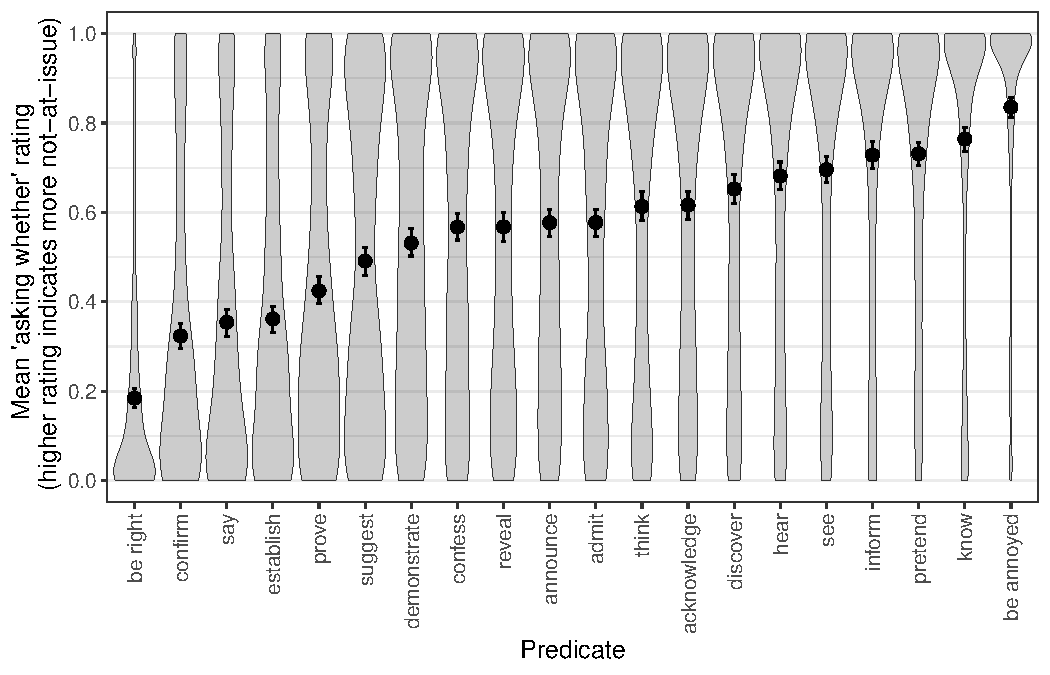
\includegraphics[width=0.7\textwidth]{../../results/main/degen-tonhauser-glossa/graphs/mean-asking-whether-ratings.pdf}

  \caption{Mean `asking whether' ratings for the contents of the clausal complements of 20 clause-embedding predicates, from \citealt{degen-tonhauser-glossa}.}
  \label{fig:dtglossa}
  \end{figure}
  

  In summary, we will investigate the questions developed above, and repeated here:
    \begin{enumerate}
      \item Can we replicate a systematic difference between the QUD-diagnostic and direct dissent, ‘yes, but’, and `asking whether' for sentence-medial appositives?
      \item Can the contrast between medial and final appositives be replicated with direct dissent, and will any of the other three diagnostics reveal a similar difference?
      \item Will we find a difference for \emph{know} between the asking-whether diagnostic and the other three?
    \end{enumerate}

  In addition, to systematically assess differences between the diagnostics, we follow \citealt{tonhauser_how_2018}, which includes a brief comparison of the `asking whether' diagnostic and another diagnostic used there, the `are you sure' diagnostic\footnote{say something about this?}.

  \begin{itemize}
    \item compare where they distinguish between the tested expressions, and where they dont
    \item the relative order between these items
    \item the spread and variation between the ratings for the items
    \item the spread and variation within the ratings for the items
  \end{itemize}

  The paper will proceed as follows:
  \begin{itemize}
    \item Section 2: exps 1--4
    \item Section 3: exps 5 and 6
    \item Section 4: General discussion
    \item Section 5: Conclusion

  \end{itemize}


\section{Assessing at-issueness}
  \subsection{QUD-diagnostic}
    The QUD diagnostic tests whether a propositional content associated with a declarative assertion (\pref{qud}B) can be interpreted as Q-at-issue by testing whether the assertion is felicitous as an answer to a preceding question that targets that content.
    \begin{itemize}
      \item show here
    \end{itemize}
    % The notion that the at-issueness of a content is related to whether it is used to address the QUD , defined explicitly in \citealt{simons_what_2010}, is labeled Q(uestion)-at-issueness in \citepos{koev_notions_2018} overview:

    \ex. \label{def:qai}%
      Q-at-issueness: \hfill (based on \citealt{simons_what_2010}: 26, \citealt{koev_notions_2018}: 2)\\
        A content $m$ is Q-at-issue in a context $c$ iff
        \a. \label{def:qai-relevant}%
          $m$ is relevant to the QUD in $c$, and
        \b.  \label{def:qai-conventional}%
          $p$ is appropriately conventionally marked relative to the QUD.
        \z. 
      \z.

      Here, $m$ may be either a propositional content or a question meaning. Relevance to the QUD is defined as follows:

      \ex. Relevance to the QUD in context $c$ \hfill (based on \citealt{simons_what_2010}: 13)
        \a. A proposition $p$ is relevant the QUD iff it contextually entails in $c$ a partial or complete answer to the QUD.
        \b. A question $q$ is relevant to the QUD, iff it has an answer that is relevant to the QUD.
        \z.
      \z.

      The QUD-diagnostic from \citealt{tonhauser_diagnosing_2012} operationalizes Q-at-issueness through naturalness judgments. It builds on two assumptions:
      \begin{enumerate}
        \item An overt question explicitly introduces a QUD.\footnote{add reference}
        \item An utterance is felicitous only if its at-issue content is relevant to the QUD (\citealt{amaral_review_2007,tonhauser_diagnosing_2012}).
      \end{enumerate}

      Koev suggests that this diagnostic is \emph{backward-looking}, because it tests whether a given content is at-issue relative to the previous discourse.

      \noindent To test whether a given content $m$ can be construed as Q-at-issue, participants are presented with a context that establishes a QUD via an overt question, followed by a response that includes $m$. For instance, \ref{qud} is used to diagnose the status of the content $m$ of the appositive RC (Greg bought a car) conveyed by B's utterance $U$, by presenting it as a response to a question $Q$ that $m$ is relevant to (What did Greg buy?), and asking a naturalness rating for $U$ as a response to $Q$.

      \ex.[\ref{qud}]
        \a.[A:] \emph{What did Greg buy?}
        \b.[B:] \emph{Greg, who bought a new car, is envied by his neighbor.}
        \z.
        Question to participants: How well does B's response fit A's question?
      \z.

      If $m$ (Greg bought a car) is interpreted as addressing the QUD, the response should receive high naturalness ratings. However, responses like (\pref{qud}B) typically receive low ratings, suggesting that $m$ is not at-issue, that is, even though $m$ is relevant to $Q$ and thereby satisfies the first part of the definition in \ref{def:qai-relevant}. The low naturalness should, therefore, reflect that $m$ is not-at-issue due to the second part of the definition in \ref{def:qai-conventional}: The low ratings for (\pref{qud}B) support the claim that appositive RCs are not appropriately conventionally marked to contribute at-issue content.

      \begin{itemize}
        \item \citealt{chen_presuppositions_2024} used this diagnostic 

        comparing  

      \end{itemize}

  \subsection{Direct dissent and `yes, but' diagnostic}
    Accordingly, the direct-dissent diagnostic \ref{dd} tests whether a proposition associated with the initial utterance (\pref{dd}A) can be interpreted as P-at-issue by testing whether it can be felicitously contradicted using \emph{no}. Relatedly, the `yes, but' diagnostic \ref{yesbut} assesses whether speakers prefer to signal agreement (using \emph{yes}) or disagreement (using \emph{no}) with the main assertion when contradicting the tested content.

    The direct dissent diagnostic \ref{dd} and the `yes, but' diagnostic \ref{yesbut} reflect the notion of P(roposal)-at-issueness, based on the assumption that at-issue content contributes to the main assertion of an utterance, which is taken to constitute a proposal to update the common ground.

     \ex. P-at-issueness: \hfill (\citealt{koev_apposition_2013,koev_notions_2018})\\
      A proposition $p$ is P-at-issue in a context $c$ iff
      \a. $p$ is a proposal in $c$ and
      \b. $p$ has not been accepted or rejected in $c$.
      \z.
    \z.

    Under this conception, the at-issue assertion is the contribution of an utterance that can be directly assented or dissented with using default discourse moves (in the sense of \citealt{farkas_reacting_2010}), for instance, using polar response particles (like English \emph{yes/no}). Conversely, non-at-issue content is assumed to be entailed by the common ground prior to the utterance in question (e.g., presupposed content, \citealt{stalnaker_presuppositions_1973,stalnaker_common_2002}), or imposed on the common ground (\citealt{murray_varieties_2014,anderbois_at-issue_2015}). Importantly, the diagnostics in \ref{dd} and \ref{yesbut} build on the assumption that non-at-issue content requires non-default discourse moves (such as revision, correction, or negotiation) to be dissented with.

    \begin{itemize}
      \item that it should be possible to signal (at least partial) agreement with the main assertion of an utterance even when contradicting is non-at-issue content. It tests whether speakers prefer signaling agreement or disagreement with the previous assertion (using \emph{yes/no}) in repsonses that contradict the content in question.

    \end{itemize}

    \begin{itemize}
      \item These two diagnostics are characterized by \citealt{koev_notions_2018} as \emph{forward-looking}, as they test whether a given content is at-issue relative to utterances in the following discourse.


      \item \citealt{syrett_experimental_2015} Their Exp. 2 found that given a choice to disagree with a preceding main clause or appositive content, participants choose disagreeing with the main clause over a medial appositive around 80\% of the time. However, for final medial RCs, this proportion is reduced to around 65\%. They conclude that final appositive clauses can compete with main clause content in the direct-dissent diagnostic, allowing these contents to be more readily interpreted as at-issue.

      \item \citealt{syrett_experimental_2015}, Exp. 2: used a variant of the direct-dissent diagnostic within a forced-choice continuation task. 
      \item utterance that included some appositive content (illustated here for a medial appositive RC)

      polarity particle \emph{no} to disagree  choice to disagree with the main clause content, or the apposistive content.
    \end{itemize}

    \ex. \a.[A] My friend Sophie, \underline{who performed a piece by Mozart,} is a classical violinist.
      \b.[B1:] No, she’s not. (target: main clause)
      \b.[B2:] No, she didn’t. (target: appositive)
      \z. \z. 

      to avoid concerns that the choice about which proposition to disagree with may be affected by the participants opinion about the content of these propositions, we instead chose a version of the direct dissent task that more directky targets the question whether disagrement using \emph{no} is acceptable, by using acceptabiltiy judgments.

  \subsection{Asking whether}
    This diagnostic tests whether a content associated with a polar question \ref{aw} can be interpreted as at-issue by testing whether informands will understand it as the main issue being asked about.

    Because the definition in \ref{def:qai} references the preceding context, \citet{koev_notions_2018} suggests that QUD-at-issueness is a backward-looking notion of at-issueness. However, overt questions may explicitly raise a QUD\footnote{add reference}, and thereby make a content Q-at-issue in the subsequent discourse. This is what is targeted by the `asking whether' diagnostic in \ref{aw} (\citealt{tonhauser_how_2018}), based on the assumption that it is the at-issue content of interrogatives that partitions the context set, as opposed to their non-at-issue content (p.502).

    \ex.[\ref{aw}]%
        \emph{Is Greg, who bought a new car, envied by his neighbor?}\smallskip
    \\ Question to participants: Is the speaker asking whether Greg bought a new car?
    \z.

    explain explain
    If participants respond "no," this suggests that the appositive content (Greg bought a new car) is not part of the at-issue content of the interrogative, providing evidence that it is not Q-at-issue. This diagnostic thus complements the QUD-diagnostic by probing the at-issueness of content from the perspective of explicitly raised questions rather than previously established ones.

    based on the assumption that it is the at-issue content of interrogatives that partitions the context set, as opposed to their non-at-issue content (\citealt{tonhauser_how_2018} p.502).


    \begin{itemize}

      \item \citealt{destruel_cross-linguistic_2015}: when German medial appositives are contradicted in the following utterance, then most participants choose to signal agreement and contrast \emph{yes, but} ($\approx 90\%$), suggesting NAI status.

      \item \citealt{tonhauser_how_2018}, Medial appositives are among the contents that get the lowest ratings for asking-whether diagnostic in their Exp.1a, suggesting that these are NAI (see also \citealt{solstad_cataphoric_2024})
    \end{itemize}
  


\section{Discussion}
  \subsection{Direction}
  \subsection{Speech-act}
  \subsection{Logical (in)dependence between contents}
    \begin{itemize}
      \item Some diagnostics, especially (dis)agreement also interact with speaker commitments

      \item if the embedded content is false participants may choose to disagree with the main assertion, not necessarily because it is interpreted as at-issue, but because it is assumed to be true, and entails that the at-issue content is false.

    \end{itemize}

  \subsection{Koev's dichotomy}
    If we contrast these notions by whether what is at-issue is determined by a declarative vs. an interrogative utterance, the asking whether test aligns more closely with the assumptions of the QUD-based notion of Q-at-issueness. However, Koev suggests that the two notions also differ in their directionality in discourse, arguing that the use of the diagnostics and defitinitions of at-issueness in the literature suggest that Q-at-issueness of a content is determined by the previous discourse (backward-looking), whereas P-at-issueness determines what will be at-issue at the point of the utterance and in subsequent discourse (forward-looking). Considering that the `asking whether' diagnostic assumes that the at-issue content of an interrogative makes a content Q-at-issue in the discourse moving forward, this suggests that the dichotomy between forward-looking P-at-issueness and backward-looking Q-at-issueness might benefit from refining it by considering all logically possible combinations between speech act (assertion vs. question) and directionality in discourse (backward vs. forward).

\nocite{*} %this is to get all the entries of the sample bibliography; delete this line for an actual Glossa submission

%\printbibliography %for use with biblatex; comment out if you use natbib
\bibliography{../at-issueness} %for use with natbib; comment out if you use biblatex, and change 'sample' by the name of your bib-file


\end{document}
